\section{Architektur}

In diesem Kapitel erfolgt die Präsentation der Architektur der visionierten Webanwendung.
Das UML-Komponentendiagramm in Abbildung \ref{Architektur} visualisiert die Bestandteile der Anwendung.  

\begin{figure}[h!]
    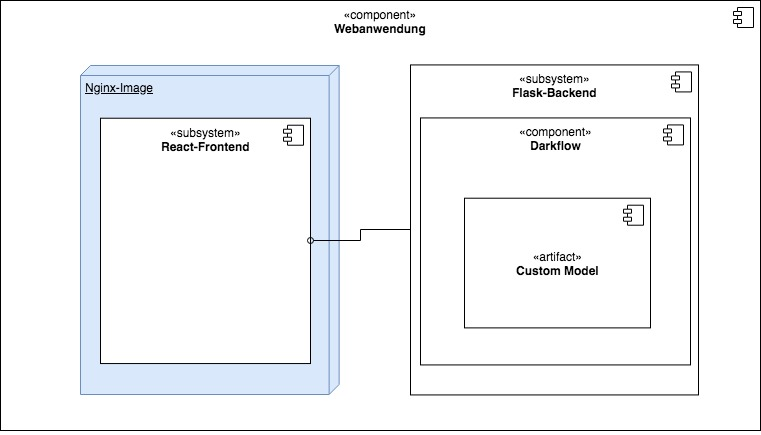
\includegraphics[width=\linewidth]{resources/images/bigdata-prak-arch_recent.jpg}
    \caption{Architektur der visionierten Webanwendung}
    \label{Architektur}
\end{figure}

Zur Identifizierung von relevanten Objekten wird die \textit{YOLO}-Architektur genutzt.
Bei \textit{YOLO} handelt es sich um ein neuronales Netz, dass zum detektieren sowie zum lokalisieren von Objekten entworfen wurde.
Die in diesem Projekt verwendete \textit{YOLO}-Implementierung heißt \textit{Darkflow}. 

Die Webanwendung basiert auf einer Client-Server-Architektur.
Auf Serverseite wird das leichtgewichtige Python-Framework \textit{Flask} genutzt.
Flask wurde mit dem Ziel entwickelt seinen Nutzern einen einfachen und schnellen Einstieg zu ermöglichen, 
jedoch mit der Möglichkeit bis hin zu komplexen Anwendungen zu skalieren (vgl. siehe \cite{palletsprojects}). 

Im Frontend kommt die von \textit{Facebook} entwickelte JavaScript-Library \textit{React} zum Einsatz.
Wie andere komponentenbasierte Frontend-Frameworks stellt auch \textit{React} einen komfortablen und schnellen 
Weg zur Erstellung von UI-Komponenten bereit (vgl. siehe \cite{react.js}). 
Die im Frontend erstellten Grafiken werden mithilfe von \textit{p5.js} erstellt.
Dabei handelt es sich wiederum um eine JavaScript-Library für die Erstellung von grafischen und interaktiven
Inhalten (vgl. siehe \cite{p5.js}). 

Sämtliche Komponenten des Systems werden mithilfe der Container\-virtualisierungs-Technologie Docker deployed.
Docker ermöglicht die Bereitstellung und den Betrieb von Linux-Containern.
Innerhalb dieser Container können Images deployed werden, die unter anderem auf \textit{Dockerhub} (\url{https://hub.docker.com/}) 
bereitgestellt werden (vgl. siehe \cite{redhat-docker}).
Im Rahmen des Projekts wird beispielsweise das offizielle Image des \textit{Nginx}-Webservers verwendet, um den 
Production-Build des Frontends bereitzustellen.



% Im Folgenden soll der Aufbau der Anwendung näher beleuchtet werden.
% Zunächst erfolgt die Präsentation des verwendeten Technologiestacks. 
% Anschließend werden die eingesetzten Komponenten vorgestellt und ein Überblick über ihre Funktionsweise geliefert.
% Für einen besseren Überblick über die Anwendung wird die Gesamtarchitektur mit Hilfe eines UML-Komponentendiagramms 
% visualisiert.

% \subsection{Architektur}

% Zur Erkennung von relevanten Objekten wird die \textit{YOLO}-Architektur genutzt.
% Bei \textit{YOLO} handelt es sich um ein Architekturmodell zur Objekterkennung.
% Die verwendete \textit{YOLO}-Implementierung heißt \textit{Darknet}. 

% % // Darkflow --> Implementiert Tensorflow

% Im Rahmen der Webanwendung wird eine Client-Server-Architektur eingesetzt. 
% Auf Serverseite wird das leichtgewichtige Framework \textit{Flask} genutzt.
% Im Frontend kommt die von \textit{Facebook} entwickelte JavaScript-Library \textit{React} zum Einsatz.
% Das Deployment erfolgt mit Hilfe der Containervirtualisierungs-Plattform \textit{Docker}.

% % des von \textit{Google} 
% % entwickelten Deep Learning - Frameworks \textit{Tensorflow} realisiert. 

% \subsection{Trainieren und Testen}

% Zur Verbesserung der Ergebnisse des vortrainierten Modells wird dieses mithilfe einer Vielzahl eigener Daten trainiert.
% Die Trainingsdaten werden zur ihrer Verwendung vorbereitet, das heißt dass die relevanten Objekte händisch 
% \textit{gelabelt} werden. Als relevante Objekte werden im Projektkontext PKWs, LKWs, Busse sowie Motorräder betrachtet.

% \subsection{Ablauf}

% Im ersten Schritt wird das aktuell öffentlich verfügbare Bild der Webcam \textit{gecrawled}. 
% Dieses wird als Input für das neuronale Netz eingesetzt und mit Hilfe des vortrainierten Modells analysiert.
% Als Ausgabe werden die auf dem Bild befindlichen, als relevant deklarierten, Objekte mit einem \textit{Confidence}-Wert
% zurückgegeben. 
% Der \textit{Confidence}-Wert stellt die Wahrscheinlichkeit dar, dass es sich um das jeweilige gekennzeichnete Objekt handelt.

